
        \documentclass[12pt]{article}
        \usepackage[utf8]{inputenc}
        \usepackage{datatool}
        \usepackage{geometry}
        \usepackage{pgfplots}
        \pgfplotsset{compat=1.18}
        \usepgfplotslibrary{polar}
        \usepackage{pgfplotstable}
        \usepackage{float}
        \usepackage{multicol}
        \usepackage[most]{tcolorbox}
        \geometry{left=1cm,right=1cm,top=2cm,bottom=2cm}
        \usepackage{hyperref}

        \DTLsetseparator{;} % Assurez-vous que cela correspond au séparateur de votre fichier CSV.
        \def\boitecouleur{gray!75!black}
        \newcommand\boite[2]{
            \begin{tcolorbox}[nobeforeafter,title=\bfseries #1,halign title=flush left,fonttitle=\bfseries,colbacktitle=\boitecouleur,coltitle=white,colback=white]%red!50!black
                #2
            \end{tcolorbox}
        }
        \begin{document}
        
\section{Résultats de AGEUGEU Beubeubeu}

    %%% debut - tableau %%%
    \boitesignature{
    \textbf{Contrôle effectué le : 15/10/2024} \\
    \textbf{Thèmes abordés : }Pythagore
    }{\begin{center}\bfseries\huge{3/5{,}5} \end{center}}

    \begin{center}
        
\begin{tabular}{|c|c|c|}
      \hline
       & \bfseries Exercice 1  & \bfseries Exercice 2  \\
      \hline
      \bfseries Points  & 1 & 2 \\
      \hline
      \bfseries Barème  & 1 & 4.5 \\
      \hline
\end{tabular}

    \end{center}

    %%% fin - tableau %%%

\begin{multicols}{2}

    %%% debut - explications %%%
    \boite{Commentaires :}{
        
            \begin{itemize}

                \item \textbf{Exercice 2} à retravailler.\\ 
                    Reprendre le cours sur cette compétence. Effectuer l'exercice sur une feuille en y inscrivant le numéro et la page d l'exercice. Remettre ce document au professeur pour correction.
                    
            
            \end{itemize}

    
    }
    %%% fin - explications %%%
    
    \columnbreak

    %%% debut - radar %%%
    
    
\begin{center}
    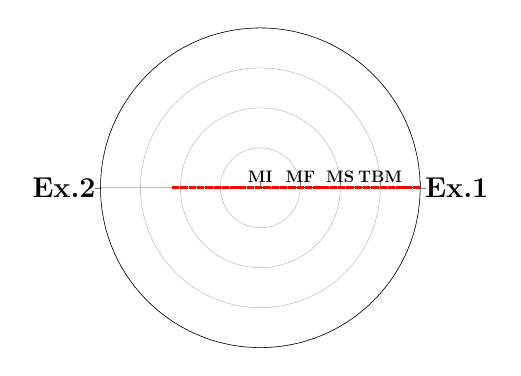
\begin{tikzpicture}[scale=0.5]
        \begin{polaraxis}[
            width=0.8\textwidth,
            xtick={0.0,180.0},
            xticklabels={\huge \bfseries Ex.1,\huge \bfseries Ex.2},
            ymin=0, ymax=100,
            ytick={0,25,50,75,100},
            yticklabels={\large \bfseries MI,\large \bfseries MF,\large \bfseries MS,\large \bfseries TBM, }
        ]
        \addplot+[mark=none,fill=blue,opacity=0.5] coordinates {
            (0.0,100.0)  (180.0,44.44444444444444)  
        } -- cycle;
        
        \addplot+[mark=none,fill=none,opacity=1,line width = 2pt,dashed,color=red] coordinates {
                    (0.0,100.0)  (180.0,55.55555555555556)  
                } -- cycle;
        
        \end{polaraxis}
    \end{tikzpicture}
\end{center}


    %%% fin - radar %%%

\end{multicols}

        \end{document}
        